% ----------------------- TODO ---------------------------
% Diese Daten müssen pro Blatt angepasst werden:
\newcommand{\NUMBER}{VHDL Vorführung}
\newcommand{\EXERCISES}{5}
% Diese Daten müssen einmalig pro Vorlesung angepasst werden:
\newcommand{\COURSE}{Grundlagen der Digitaltechnik}
\newcommand{\TOPIC}{}
\newcommand{\DATE}{10.06.2022}
% ----------------------- TODO ---------------------------

\documentclass[a4paper]{scrartcl}

\usepackage[utf8]{inputenc}
\usepackage[ngerman]{babel}
\usepackage{amsmath}
\usepackage{amssymb}
\usepackage{fancyhdr}
\usepackage{color}
\usepackage{graphicx}
\usepackage{lastpage}
\usepackage{listings}
\usepackage{tikz}
\usepackage{pdflscape}
\usepackage{subfigure}
\usepackage{float}
\usepackage{polynom}
\usepackage{hyperref}
\usepackage{tabularx}
\usepackage{forloop}
\usepackage{geometry}
\usepackage{listings}
\usepackage{fancybox}
\usepackage{tikz}
\usepackage{algpseudocode,algorithm,algorithmicx}

%Definiere Let-Command für algorithmen
\newcommand*\Let[2]{\State #1 $\gets$ #2}

\input kvmacros

%Größe der Ränder setzen
\geometry{a4paper,left=3cm, right=3cm, top=3cm, bottom=3cm}

%Kopf- und Fußzeile
\pagestyle {fancy}
\fancyhead[L]{\COURSE}
\fancyhead[R]{\DATE}

\fancyfoot[L]{}
\fancyfoot[C]{}
\fancyfoot[R]{Seite \thepage /\pageref*{LastPage}}
\setlength{\parindent}{0pt}

%Formatierung der Überschrift, hier nichts ändern
\def\header#1#2{
  \begin{center}
    {\Large Labor: #1 \TOPIC}\\
    {(Datum #2)}
  \end{center}
}


\begin{document}


\header{ \NUMBER}{\DATE}

\section*{Aufgabe 1: Installtion}
Für die Simulation unserer VHDL Designs, sowie die Auswertung unsere Simulationsergebnisse brauchen wir zwei Tools. GHDL
ein Open Source ``analyzer, compiler, simulator and (experimental) synthesizer for VHDL''. GHDL erzeugt sogenannte ``Waveforms''
(Signalgraphen), damit wir diese anschauen können, brauchen wir einen Viewer: gtkwave.\\

\textbf{GHDL}
\begin{itemize}
  \item Für Linux:
  \begin{itemize}
    \item Nutze einfach deinen System-Package-Manager
    \item z.B. auf Debian: \texttt{sudo apt install ghdl}
  \end{itemize}
  \item Für Windows/MacOS:
  \begin{itemize}
    \item https://github.com/ghdl/ghdl
    \item Gehe zu: Releases
    \item Downloade ein für dein OS passendes Paket
    \begin{itemize}
      \item für Windows z.B.: ghdl-UCRT64.zip
      \item für MacOS z.B.: ghdl-macos-11-llvm.tgz
    \end{itemize}
  \end{itemize}
\end{itemize}

\textbf{gtkwave}
\begin{itemize}
  \item Für Linux:
  \begin{itemize}
    \item Nutze einfach deinen System-Package-Manager
    \item z.B. auf Debian: \texttt{sudo apt install gtkwave}
  \end{itemize}
  \item Für Windows/MacOS:
  \begin{itemize}
    \item https://sourceforge.net/projects/gtkwave/files/
    \item Scrolle durch die Liste und finde ein für dich richtiges Paket
    \begin{itemize}
      \item für Windows z.B.: gtkwave-3.3.100-bin-win64
      \item für MacOS z.B.: gtkwave-3.3.107-osx-app
    \end{itemize}
  \end{itemize}
\end{itemize}


\section*{Bespielaufgabe 2: Full-Adder Beispiel}
\subsection*{a) Simulation}
Um dich an die beiden neuen Tools zu gewöhnen, legen wir mal mit einer Beispielaufgabe an.
Ähnlich wie wir es in manchen vorherigen Laboren in Logisim gemacht haben, wollen wir auch in VHDL
für jede Komponente in VHDL eine Testkomponente, welche dies Komponente testet anlegen.\\

Das Beispiel besteht aus zwei Dateien. 
\begin{itemize}
  \item \texttt{adder.vhd}: Implementiert einen 1-Bit Full-Adder.
  \item \texttt{tb\_adder.vhd}: Ist die Testbench für den 1-Bit Full-Adder.
\end{itemize}
Schaue in beide Files und versuche mit den Informationen, die du in der Einführung zu VHDL bekommen hast zu verstehen, was dort vor sich geht.

Versuch folgenden Fragen zu beantworten:
\begin{itemize}
  \item Hat der 1-Bit Full-Adder Ein-/Ausgänge?
  \item Was passiert intern im 1-Bit Full-Adder?
  \item Ist die Testbench mit dem Full-Adder verschalten? Wenn ja wie?
  \item Was macht die Testbench?
  \item Hat die die Testbench Ein-/Ausgänge? Wenn ja warum, wenn nein warum nicht?
  \item Was versuchen wir zu addieren?
\end{itemize}

Wenn du denkst du hast die beiden Komponente verstanden versuche das Beispiel zu simulieren und die Ergebnisse anzuschauen.
Für die Simulation kann unter Linux einfach das mitgelieferte Makefile ausgeführt werden. Für Windows/MacOS muss ein Script mit den folgenden Commands angelegt werden (oder 
die CMDs nacheinander ausgeführt werden).
Stelle sicher, dass die Befehle im Verzeichnis des VHDL-Projekts ausgeführt wird:\\
Windows/MacOS:
\begin{itemize}
  \item $<$PathToExe$>$/ghdl -a --std=08 adder.vhd tb\_adder.vhd
	\item $<$PathToExe$>$/ghdl -e --std=08 adder\_tb
	\item $<$PathToExe$>$/ghdl -r --std=08 adder\_tb --wave=wave.ghw --stop-time=50ns
	\item $<$PathToExe$>$/gtkwave wave.ghw
\end{itemize}
Linux:
\begin{itemize}
  \item make
	\item gtkwave wave.ghw
\end{itemize}

Mit dem \texttt{gtkwave} Befehl sollte ein Fenster aufgegangen sein, in welchem man nun die Simulationsergebnisse anschauen kann. Analysiere dort die Signale.
% \begin{center}
  \begin{figure}[h]
    \centering
    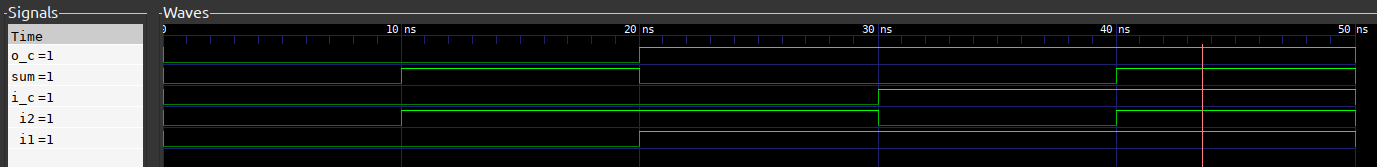
\includegraphics[width=10cm]{gtkwave.png}
  \end{figure}
% \end{center}
  


\subsection*{b) Design vs. Simulation}
Mit dem GHDL-Compiler kann man zwar seine VHDL Designs simulieren, aber man kann damit nur experimentell Binär-Files erzugen, die man zum Beispiel in ein FPGA programmieren könnte. 
Um aus einem VHDL Design eine Datei zu erzeugen, welche in ein FPGA geladen werden kann, benötigt man typischerweise IDE des Herstellers (z.B. Xilinx Vivado o.
Intel Quartus). Diese IDEs integrieren meist direkt einen Simulator, so dass man in einer großen IDE entwickeln, simulieren und das Binär-File erstellen kann. Diese
Suites sind typischerweise mehrere Gigabyte groß und nicht umsonst.

\subsection*{c)}
VHDL ist eine Hardwarebeschreibungssprache und damit erstmal nicht zu verwechseln mit einer Programmiersprache. Unsere adder.vhd beschreibt Hardware und erstmal keinen Algorithmus 
in SW. Durch die Möglichkeit der Simulation, die wir mit der Testbench nutzen, kann in VHDL aber dennoch Datenverarbeitung stattfinden (dadurch ist VHDL zusammen mit einem
Simulator z.B. GHDL turing vollständig).

Um aus einer VHDL Implementierung echte HW zu erzeugen  muss ein VHDL Design ``synthethisiert'' werden (d.h. es muss in eine niedrigere Abstraktionschicht gebracht werden).
Z.B. aus VHDL nach RTL (Register Transfer Logik)). Dies wird
benötigt, um daraus ein Design für Lithografiemasken für einen Chip oder das Binär-File für ein FPGA zu erzeugen. 

Es sind aber nicht alle .vhd Files synthethisierbar.
Fragen:
\begin{itemize}
  \item Ist der adder.vhd synthethisierbar? Warum?
  \item Ist der tb\_adder.vhd synthethisierbar? Warum?
\end{itemize}


\section*{Aufgabe 3: Der 4 Bit-Adder}
Versuche mit der 1-Bit Adder Komponente durch Verschaltung einen 4-Bit Adder zu erstellen. Erstelle auch hier für eine Testbench und führe eine Simulation durch.
Analysiere die Ergebnisse mit  gtkwave.

\section*{Aufgabe 4: ALU (Bonusaufgabe für Zuhause)}
Modelliere und simuliere die ALU aus Labor 2 mit VHDL. Gehe hier Schritt für Schritt vor:\\
\begin{itemize}
  \item Erstelle Entities für jeden Block (z.B. für das 8-Bit OR).
  \item Erstelle Testbenches für jeden Block
  \item Simuliere/Teste jeden einzelnen Block auf korrekte Verschaltung
  \item Verschalte die Blöcke in einer Top-Level Entity
  \item Erstelle eine Testbench für die Top-Level Entity und simuliere diese
\end{itemize}


\end{document}
%%% Local Variables:
%%% mode: latex
%%% TeX-master: t
%%% End: